\chapter{O controle estatístico de processos}
\label{chap:controle_estatistico_de_processos}


%------------------------------------------------------------------

\section{Ferramentas}
\label{sec:controle_estatistico_sec1}

\subsection{Diagrama de Correlação}
É utilizado de forma a verificar a relação dos problemas/defeitos encontrados com relação ao tempo (correlação temporal) ou relação entre problemas e suas possíveis causas (correlação causal). É uma ferramenta onde os dados são transformados em informações úteis ao direcionamento das análises de problemas pelo pessoal da linha de frente.

\subsection{Histogramas}
É uma ferramenta que apresenta os dados de forma gráfica de forma a simplificar a comparação de suas frequências de ocorrência. Muitas vezes o histograma pode ser gerado no chão de fábrica durante a produção.

\subsection{Cartas de Controle de Processos}
Essa ferramenta tem o objetivo de manter o controle de um processo através do acompanhamento do comportamento de uma ou várias variáveis importantes deste processo.

\subsection{Folhas de Verificação}
Esta ferramenta é utilizada de forma a não se esquecer de empregar as ferramentas citadas anteriormente. As folhas de verificação são conhecidas também como Checklist e são aplicadas para verificação de procedimentos de segurança, atividades e cumprimento das etapas do processo produtivo.

\subsection{Diagrama de Ishikawa}
Também conhecido como Diagrama de Causa e Efeito, neste diagrama, que possui formato de um peixe, coloca-se na "cabeça do peixe" o efeito gerado, e nas "espinhas" colocam-se as causas que originaram esse efeito. Estas causas são separadas por categorias: método, meio ambiente, mão de obra, medida, máquinas e material.

\subsection{Análise de Pareto}
Trata da relação 80/20, onde, por exemplo, 80\% dos problemas de qualidade concentram-se nos 20\% de itens fabricados, ou 80\% das falhas ocorrem devido a 20\% das causas prováveis dessas falhas. É um gráfico de barros que ordena as frequências das ocorrências em ordem decrescente, permitindo assim a identificação de problemas vitais e também a eliminação de futuras perdas. 

\subsection{Diagrama de Processos}
Esse diagrama é utilizado para fazer uma listagem de todas as fases do processo de forma a facilitar a visualização e compreensão. São utilizados símbolos para identificar o que ocorre em cada fase, além de sinalizar o tempo que leva para cada uma delas.


%------------------------------------------------------------------
\section{Aplicação Prática}
\label{sec:controle_estatistico_aplicacao}
As ferramentas que são aplicadas na SunBurn são as seguintes: Diagrama de Ishikawa, Diagrama de Correlação e Checklist.
Na Figura \ref{fig:ishikawa_aplicacao} tem-se o Diagrama de Ishikawa onde o efeito analisado é a parada de produção de energia do inversor, e as causas são divididas entre, material, máquinas, medida, meio ambiente, mão de obra e método.
Já nas Figuras \ref{fig:correlacao1_aplicacao} e \ref{fig:correlacao2_aplicacao} tem-se os Diagramas de Correlação relacionando a irradiação com a potência gerada. Na Figura \ref{fig:correlacao1_aplicacao} tem-se alguns pontos onde a potência gerada está acima da irradiação detectada, logo, isso significa que o tracker do piranômetro está parado e os outros trackers estão operando bem.
E na Figura \ref{fig:correlacao2_aplicacao} alguns pontos onde a potência gerada é inferior a irradiação detectada, significa que o tracker do piranômetro está operando normalmente e a maioria, ou alguns seguimentos dos trackers estão parados, só irá apresentar uma potência alta meio dia devido ao alinhamento das placas com o Sol.  
E por fim, para garantir que as demais ferramentas sejam utilizadas, tem-se na Figura \ref{fig:checklist_aplicacao} o checklist aplicado para verificação das atividades executadas na SunBurn. Nesse checklist verifica-se a manutenção nos autotransformadores, disjuntores e para-raios. Esses são apenas algumas das análises realizadas pela empresa, porém há várias outras dependendo da atividade realizada.

\begin{figure}[H]
    \caption{Diagrama de Ishikawa, análise na parada de produção de energia do inversor.} %!ALTERAR A IMAGEM POIS FALTA LEGENDA NO EIXO Y
    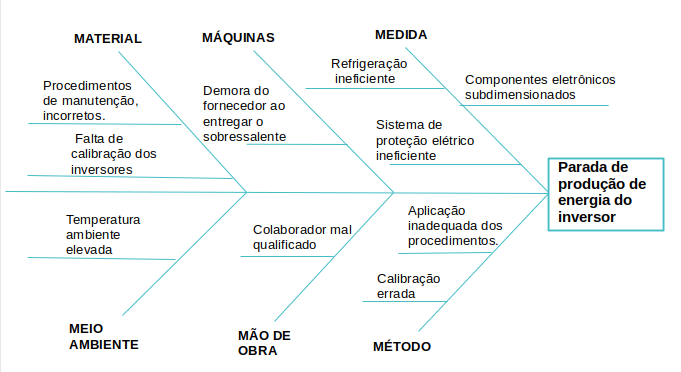
\includegraphics[width=1\textwidth]{images/ishikawa_aplicacao.png}
    \caption*{Fonte: SunBurn.}
    \label{fig:ishikawa_aplicacao}
  \end{figure}

  
  \begin{figure}[H]
    \caption{Diagrama de Correlação} %!ALTERAR A IMAGEM POIS FALTA LEGENDA NO EIXO Y
    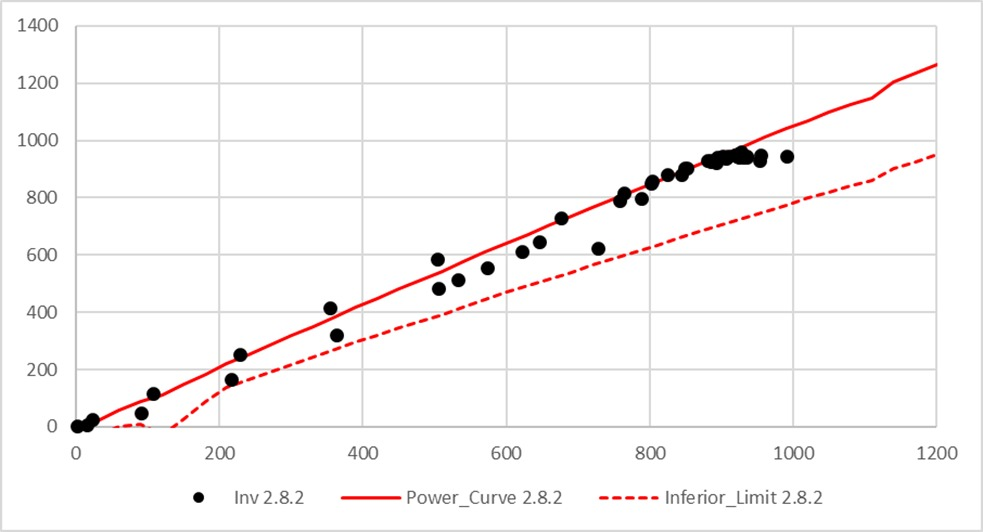
\includegraphics[width=1\textwidth]{images/correlacao_1.jpeg}
    \caption*{Fonte: SunBurn.}
    \label{fig:correlacao1_aplicacao}
  \end{figure}

  
  \begin{figure}[H]
    \caption{Diagrama de Correlação.} %!ALTERAR A IMAGEM POIS FALTA LEGENDA NO EIXO Y
    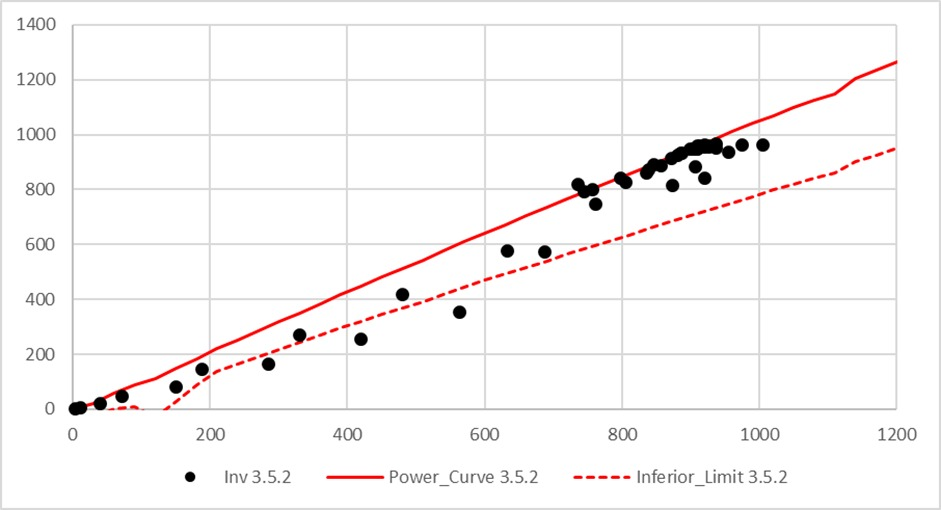
\includegraphics[width=1\textwidth]{images/correlacao_2.jpeg}
    \caption*{Fonte: SunBurn.}
    \label{fig:correlacao2_aplicacao}
  \end{figure}

  
  \begin{figure}[H]
    \caption{Checklist aplicado a Operação e Manutenção.} %!ALTERAR A IMAGEM POIS FALTA LEGENDA NO EIXO Y
    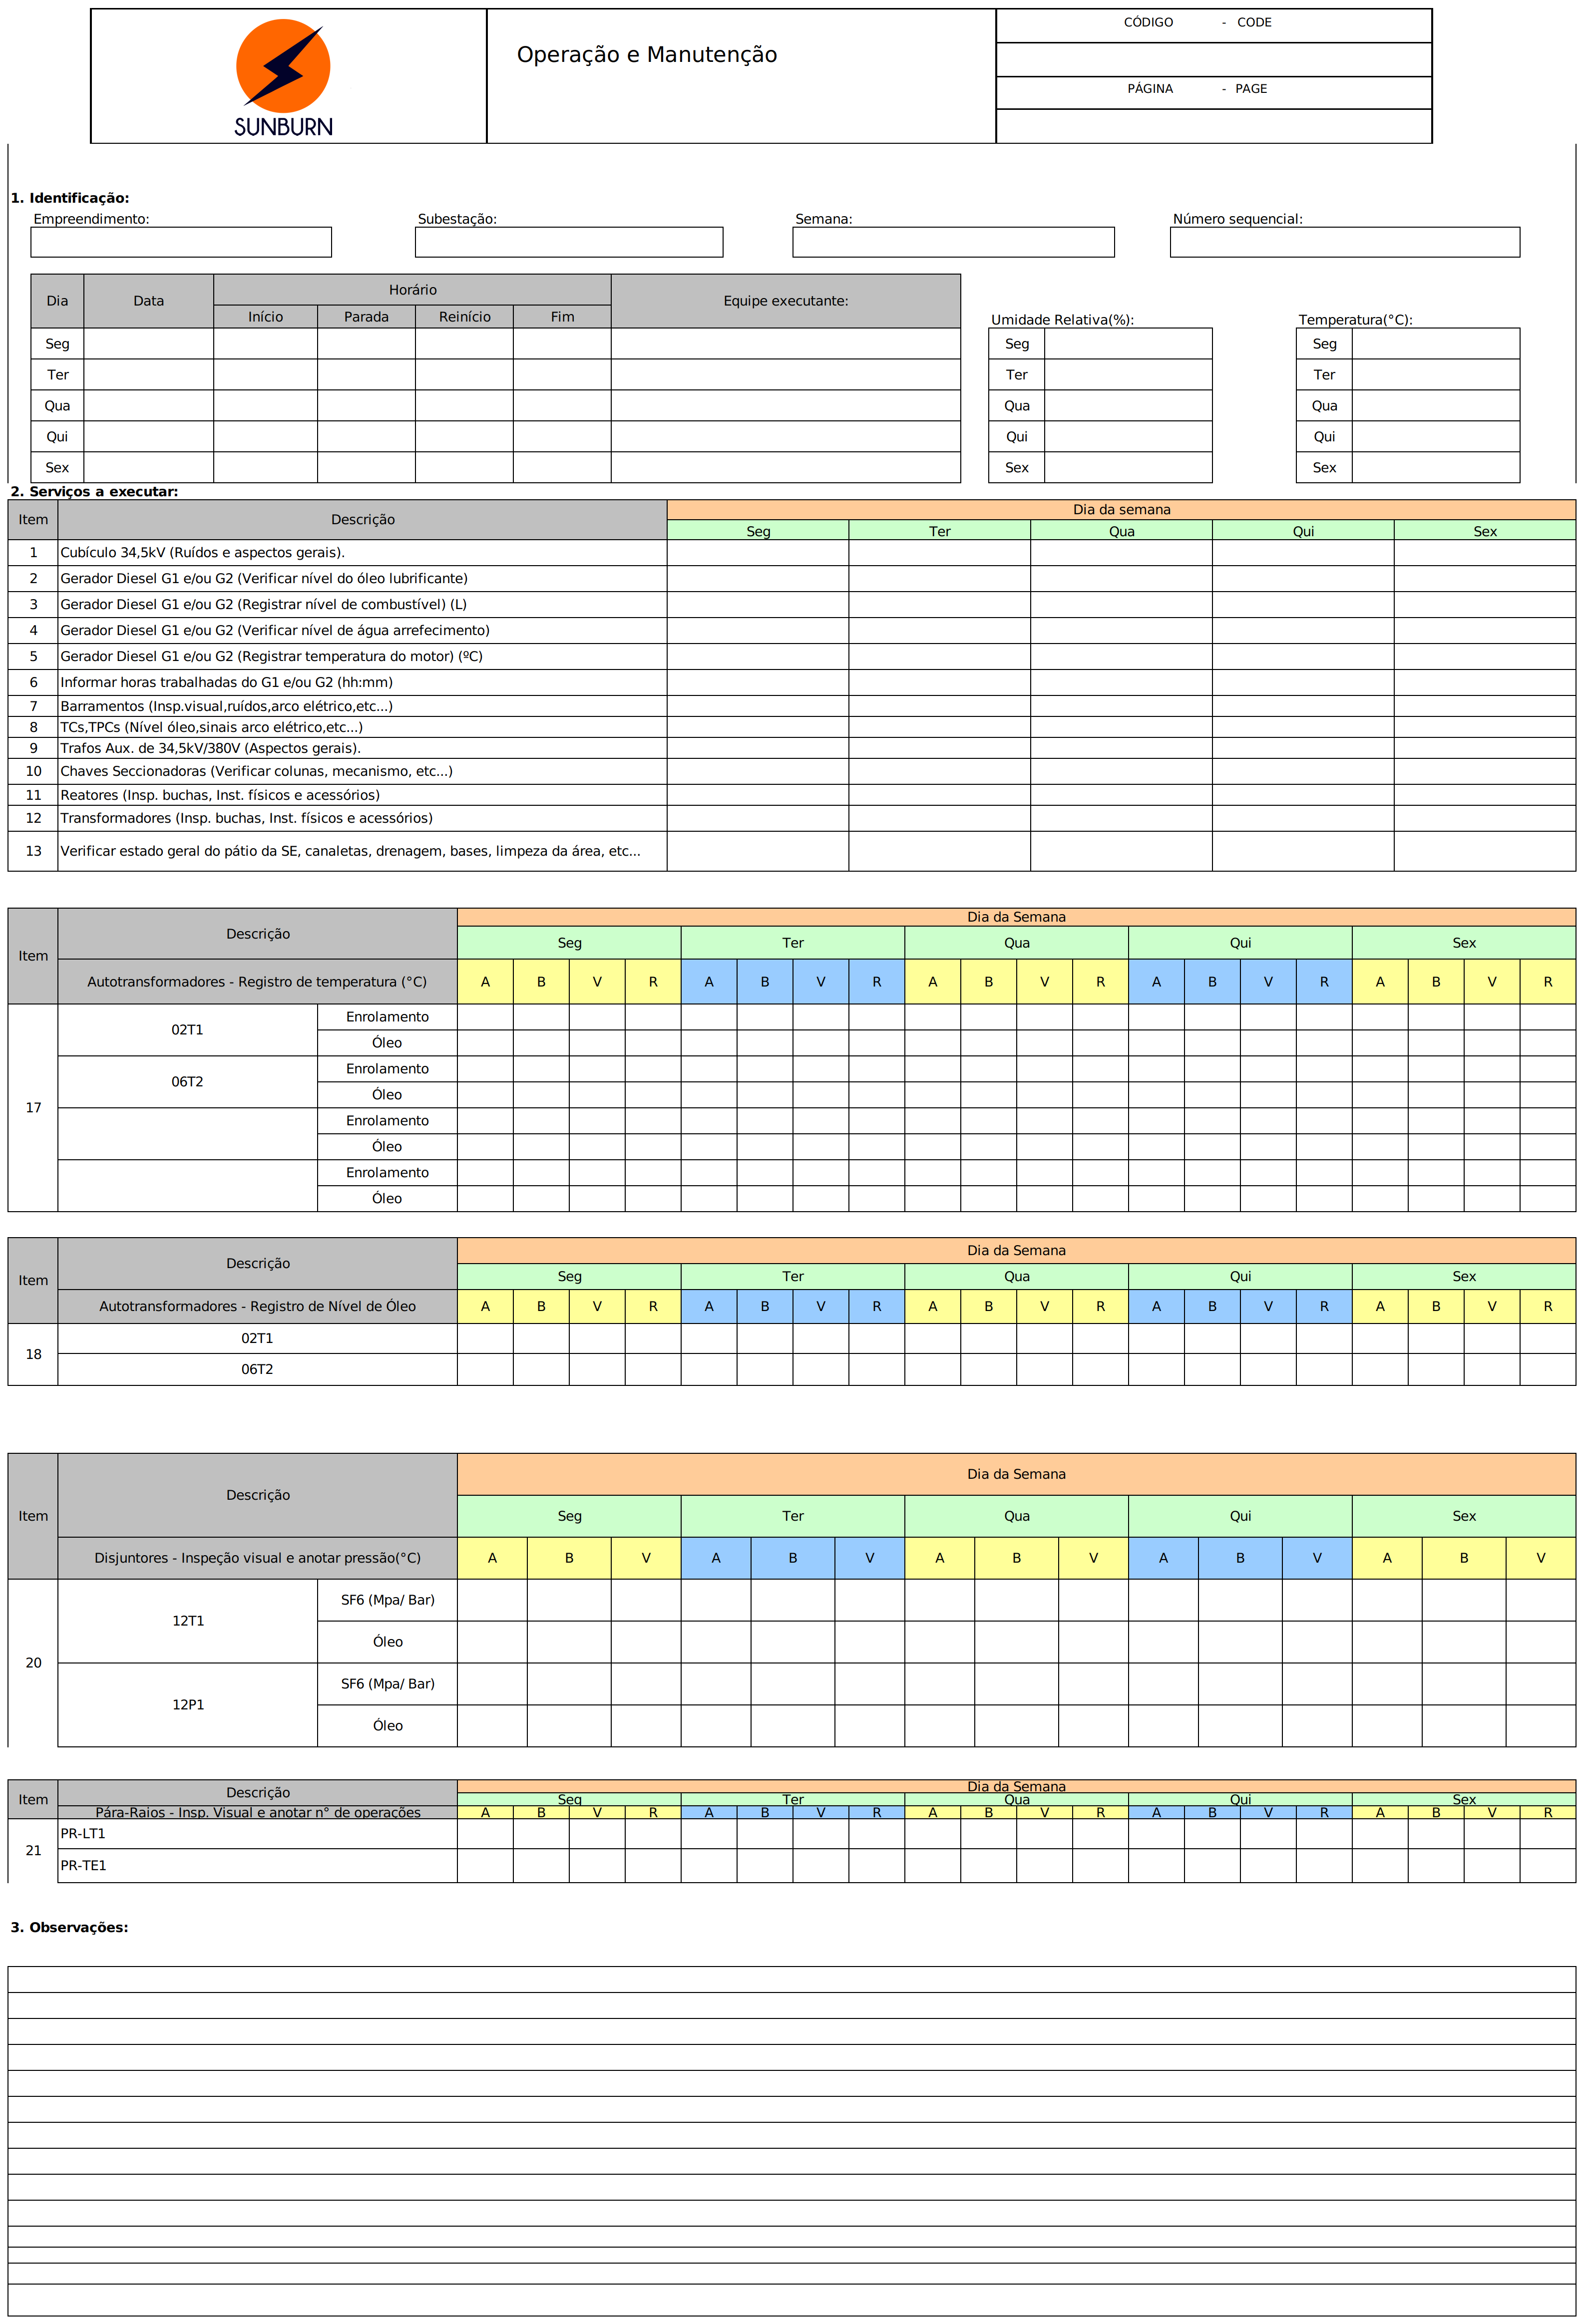
\includegraphics[width=1\textwidth]{images/checklist_aplicacao.png}
    \caption*{Fonte: SunBurn.}
    \label{fig:checklist_aplicacao}
  \end{figure}
  